\documentclass{article}

\usepackage{amsmath, amssymb, amsfonts}
\usepackage{fancyvrb}
\usepackage{graphicx}

\newcommand{\wt}{\widetilde}
\newcommand{\inner}[2]{\langle #1, #2 \rangle}

\author{Matthew Dupraz}
\title{Homework 10}

\begin{document}
	
\maketitle

\subsection*{(a)}
Let $P = LL^T$, where $L$ is the lower triangular Cholesky factor
of $P$. Let $Ax = b$ be a linear system of equations, consider
$\wt{A} = L^{-1}AL^{-T}$, $\wt{b} = L^{-1}b$.
Then the solution $\wt{x}$ to $\wt{A}\wt{x} = \wt{b}$
satisfies
\begin{equation*}
	L^{-1}AL^{-T}\wt{x} = L^{-1}b \iff AL^{-T}\wt{x} = b
\end{equation*}
Hence $L^{-T}\wt{x}$ is a solution to the equation $Ax = b$, and
since $A$ is invertible, this solution is unique, hence
$x = L^{-T}\wt{x} \iff \wt{x} = L^Tx$.

\subsection*{(b)}
The gradient method applied to the system $\wt{A}\wt{x} = \wt{x}$
gives us
\begin{align*}
	\wt{x}^{(k+1)} &= \wt{x} + \alpha_k\left(\wt{b} - \wt{A}
	\wt{x}^{(k)}\right)\\
	L^{-T}\wt{x}^{(k+1)} &= L^{-T}\wt{x} + \alpha_k\left(
	L^{-T}\wt{b} - L^{-T}\wt{A} \wt{x}^{(k)}\right)\\
	x^{(k+1)} &= x^{(k)} + \alpha_k\left(
	P^{-1}b - P^{-1}Ax^{(k)}\right)\\
	x^{(k+1)} &= x^{(k)} + \alpha_kP^{-1}\left(
	b - Ax^{(k)}\right).
\end{align*}

Let $\wt{r}^{(k)} = \wt{b} - \wt{A}\wt{x}^{(k)}$, we have that
\begin{align*}
	\wt{r}^{(k)} &= L^{-1}b - L^{-1}AL^{-T}L^{T}x^{k}\\
	&= L^{-1}(b - Ax^{k})\\
	&= L^{-1}r^{k},
\end{align*}
and so
\begin{align*}
	\alpha_k &= \frac{\inner{\wt{r}^{(k)}}{\wt{r}^{(k)}}}
	{\inner{\wt{A}\wt{r}^{(k)}}{\wt{r}^{(k)}}}
	= \frac{\inner{L^{-1}r^{(k)}}{L^{-1}r^{(k)}}}
	{\inner{L^{-1}AL^{-T}L^{-1}r^{(k)}}{L^{-1}r^{(k)}}}\\
	&= \frac{\inner{L^{-T}L^{-1}r^{(k)}}{r^{(k)}}}
	{\inner{AL^{-T}L^{-1}r^{(k)}}{L^{-T}L^{-1}r^{(k)}}}\\
	&= \frac{\inner{P^{-1}r^{(k)}}{r^{(k)}}}{\inner{AP^{-1}r^{(k)}}
	{P^{-1}r^{(k)}}}
\end{align*}

\subsection*{(c)}

We have that for any $k \in \mathbb{N}$,
\begin{align*}
	\inner{r^{(k)}}{r^{(k+1)}}_{P^{-1}} &= 
	\inner{r^{(k)}}{(I_n - \alpha AP^{-1})r^{(k)}}_{P^{-1}}\\
	&= \inner{r^{(k)}}{r^{(k)}}_{P^{-1}} - \alpha_k
	\inner{r^{(k)}}{AP^{-1}r^{(k)}}_{P^{-1}}\\
	&= \inner{P^{-1}r^{(k)}}{r^{(k)}} - \alpha_k
	\inner{P^{-1}r^{(k)}}{AP^{-1}r^{(k)}}\\
	&= 0
\end{align*}

\subsection*{(d)}

Below follows my implementation of the preconditioned gradient
method in \textsc{Matlab}.
\begin{Verbatim}[frame=single,
	label=\textsc{Matlab} code - pGrad.m]
% Preconditioned gradient method
function [x, n_iter, res] = pGrad(A, b, P_inv, tol)
	x = zeros(size(b));
	r = b - A*x;
	res = norm(r);
	n_iter = 0;
	norm_b = norm(b);
	while (res(end) > tol*norm_b)
		n_iter = n_iter + 1;

		Pr = P_inv(r);
		APr = A*Pr;
		alpha = (Pr'*r)/(Pr'*APr);
		x = x + alpha*Pr;
		r = r - alpha*APr;

		res = [res, norm(b-A*x)];
	end
end
\end{Verbatim}

When applied to the following system:
\begin{equation*}
	A = 
	\begin{bmatrix}
		2 & -1 & 0\\
		-1 & 2 & -1\\
		0 & -1 & 2
	\end{bmatrix},
	~~
	b =
	\begin{bmatrix}
		1\\ 0\\ 1
	\end{bmatrix}
\end{equation*}
with no preconditioner, the method converged in $40$
iterations.\footnote{See part (e) for the code used to obtain this
result.}

\subsection*{(e)}

We applied the method to the same system with three different 
preconditioners, below follow plots of the norms of residues against
the number of iterations with three different preconditioners.

\begin{center}
	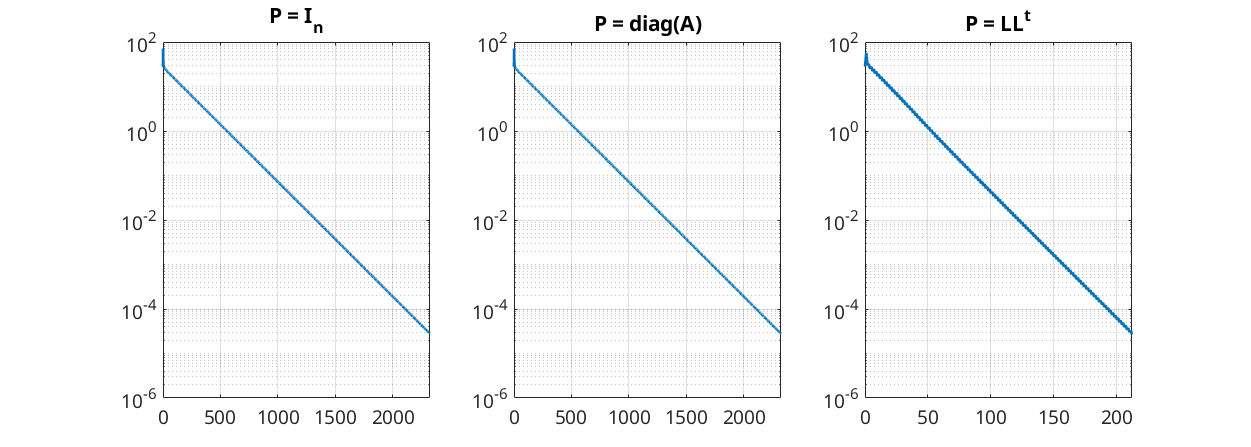
\includegraphics[width=\textwidth]{figure.png}
\end{center}

Below follows the code used to get these plots

\begin{Verbatim}[frame=single,
	label=\textsc{Matlab} code - main.m]
% Part (d)
A = [2 -1 0; -1 2 -1; 0 -1 2];
b = [1; 0; 1];
[~, n_iter] = pGrad(A, b, @(r) r, 10^(-6));

fprintf("Number of iterations: %g\n", ...
    n_iter);

% Part (e)
A = delsq(numgrid('S', 30));
b = ones(size(A,1),1);

P = speye(size(A));
[~, n_iter, res] = pGrad(A, b, @(r) P\r, 10^(-6));
subplot(1, 3, 1);
semilogy(0:n_iter, res, 'LineWidth', 2);
title('P = I_n');
grid on;
set(gca, 'FontSize', 14);

P = diag(diag(A));
[~, n_iter, res] = pGrad(A, b, @(r) P\r, 10^(-6));
subplot(1, 3, 2);
semilogy(0:n_iter, res, 'LineWidth', 2);
title('P = diag(A)');
grid on;
set(gca, 'FontSize', 14);


L = ichol(A);
[~, n_iter, res] = pGrad(A, b, @(r) L'\(L\r), 10^(-6));
subplot(1, 3, 3);
semilogy(0:n_iter, res, 'LineWidth', 2);
title('P = LL^t')
grid on;
set(gca, 'FontSize', 14);

\end{Verbatim}

\end{document}


